% Options for packages loaded elsewhere
\PassOptionsToPackage{unicode}{hyperref}
\PassOptionsToPackage{hyphens}{url}
\PassOptionsToPackage{dvipsnames,svgnames,x11names}{xcolor}
%
\documentclass[
  a4paperpaper,
  DIV=11,
  numbers=noendperiod]{scrartcl}

\usepackage{amsmath,amssymb}
\usepackage{iftex}
\ifPDFTeX
  \usepackage[T1]{fontenc}
  \usepackage[utf8]{inputenc}
  \usepackage{textcomp} % provide euro and other symbols
\else % if luatex or xetex
  \usepackage{unicode-math}
  \defaultfontfeatures{Scale=MatchLowercase}
  \defaultfontfeatures[\rmfamily]{Ligatures=TeX,Scale=1}
\fi
\usepackage{lmodern}
\ifPDFTeX\else  
    % xetex/luatex font selection
    \setmainfont[]{Ebrima}
\fi
% Use upquote if available, for straight quotes in verbatim environments
\IfFileExists{upquote.sty}{\usepackage{upquote}}{}
\IfFileExists{microtype.sty}{% use microtype if available
  \usepackage[]{microtype}
  \UseMicrotypeSet[protrusion]{basicmath} % disable protrusion for tt fonts
}{}
\makeatletter
\@ifundefined{KOMAClassName}{% if non-KOMA class
  \IfFileExists{parskip.sty}{%
    \usepackage{parskip}
  }{% else
    \setlength{\parindent}{0pt}
    \setlength{\parskip}{6pt plus 2pt minus 1pt}}
}{% if KOMA class
  \KOMAoptions{parskip=half}}
\makeatother
\usepackage{xcolor}
\usepackage[top=20mm,left=20mm,heightrounded]{geometry}
\setlength{\emergencystretch}{3em} % prevent overfull lines
\setcounter{secnumdepth}{-\maxdimen} % remove section numbering
% Make \paragraph and \subparagraph free-standing
\makeatletter
\ifx\paragraph\undefined\else
  \let\oldparagraph\paragraph
  \renewcommand{\paragraph}{
    \@ifstar
      \xxxParagraphStar
      \xxxParagraphNoStar
  }
  \newcommand{\xxxParagraphStar}[1]{\oldparagraph*{#1}\mbox{}}
  \newcommand{\xxxParagraphNoStar}[1]{\oldparagraph{#1}\mbox{}}
\fi
\ifx\subparagraph\undefined\else
  \let\oldsubparagraph\subparagraph
  \renewcommand{\subparagraph}{
    \@ifstar
      \xxxSubParagraphStar
      \xxxSubParagraphNoStar
  }
  \newcommand{\xxxSubParagraphStar}[1]{\oldsubparagraph*{#1}\mbox{}}
  \newcommand{\xxxSubParagraphNoStar}[1]{\oldsubparagraph{#1}\mbox{}}
\fi
\makeatother


\providecommand{\tightlist}{%
  \setlength{\itemsep}{0pt}\setlength{\parskip}{0pt}}\usepackage{longtable,booktabs,array}
\usepackage{calc} % for calculating minipage widths
% Correct order of tables after \paragraph or \subparagraph
\usepackage{etoolbox}
\makeatletter
\patchcmd\longtable{\par}{\if@noskipsec\mbox{}\fi\par}{}{}
\makeatother
% Allow footnotes in longtable head/foot
\IfFileExists{footnotehyper.sty}{\usepackage{footnotehyper}}{\usepackage{footnote}}
\makesavenoteenv{longtable}
\usepackage{graphicx}
\makeatletter
\newsavebox\pandoc@box
\newcommand*\pandocbounded[1]{% scales image to fit in text height/width
  \sbox\pandoc@box{#1}%
  \Gscale@div\@tempa{\textheight}{\dimexpr\ht\pandoc@box+\dp\pandoc@box\relax}%
  \Gscale@div\@tempb{\linewidth}{\wd\pandoc@box}%
  \ifdim\@tempb\p@<\@tempa\p@\let\@tempa\@tempb\fi% select the smaller of both
  \ifdim\@tempa\p@<\p@\scalebox{\@tempa}{\usebox\pandoc@box}%
  \else\usebox{\pandoc@box}%
  \fi%
}
% Set default figure placement to htbp
\def\fps@figure{htbp}
\makeatother
% definitions for citeproc citations
\NewDocumentCommand\citeproctext{}{}
\NewDocumentCommand\citeproc{mm}{%
  \begingroup\def\citeproctext{#2}\cite{#1}\endgroup}
\makeatletter
 % allow citations to break across lines
 \let\@cite@ofmt\@firstofone
 % avoid brackets around text for \cite:
 \def\@biblabel#1{}
 \def\@cite#1#2{{#1\if@tempswa , #2\fi}}
\makeatother
\newlength{\cslhangindent}
\setlength{\cslhangindent}{1.5em}
\newlength{\csllabelwidth}
\setlength{\csllabelwidth}{3em}
\newenvironment{CSLReferences}[2] % #1 hanging-indent, #2 entry-spacing
 {\begin{list}{}{%
  \setlength{\itemindent}{0pt}
  \setlength{\leftmargin}{0pt}
  \setlength{\parsep}{0pt}
  % turn on hanging indent if param 1 is 1
  \ifodd #1
   \setlength{\leftmargin}{\cslhangindent}
   \setlength{\itemindent}{-1\cslhangindent}
  \fi
  % set entry spacing
  \setlength{\itemsep}{#2\baselineskip}}}
 {\end{list}}
\usepackage{calc}
\newcommand{\CSLBlock}[1]{\hfill\break\parbox[t]{\linewidth}{\strut\ignorespaces#1\strut}}
\newcommand{\CSLLeftMargin}[1]{\parbox[t]{\csllabelwidth}{\strut#1\strut}}
\newcommand{\CSLRightInline}[1]{\parbox[t]{\linewidth - \csllabelwidth}{\strut#1\strut}}
\newcommand{\CSLIndent}[1]{\hspace{\cslhangindent}#1}

\usepackage{scrlayer-scrpage}
\rohead{Fiche protocole}
\lofoot{Projet CEPOCLIM, 2025. CC BY-NC-ND}
\KOMAoption{captions}{tableheading}
\makeatletter
\@ifpackageloaded{tcolorbox}{}{\usepackage[skins,breakable]{tcolorbox}}
\@ifpackageloaded{fontawesome5}{}{\usepackage{fontawesome5}}
\definecolor{quarto-callout-color}{HTML}{909090}
\definecolor{quarto-callout-note-color}{HTML}{0758E5}
\definecolor{quarto-callout-important-color}{HTML}{CC1914}
\definecolor{quarto-callout-warning-color}{HTML}{EB9113}
\definecolor{quarto-callout-tip-color}{HTML}{00A047}
\definecolor{quarto-callout-caution-color}{HTML}{FC5300}
\definecolor{quarto-callout-color-frame}{HTML}{acacac}
\definecolor{quarto-callout-note-color-frame}{HTML}{4582ec}
\definecolor{quarto-callout-important-color-frame}{HTML}{d9534f}
\definecolor{quarto-callout-warning-color-frame}{HTML}{f0ad4e}
\definecolor{quarto-callout-tip-color-frame}{HTML}{02b875}
\definecolor{quarto-callout-caution-color-frame}{HTML}{fd7e14}
\makeatother
\makeatletter
\@ifpackageloaded{caption}{}{\usepackage{caption}}
\AtBeginDocument{%
\ifdefined\contentsname
  \renewcommand*\contentsname{Table des matières}
\else
  \newcommand\contentsname{Table des matières}
\fi
\ifdefined\listfigurename
  \renewcommand*\listfigurename{Liste des Figures}
\else
  \newcommand\listfigurename{Liste des Figures}
\fi
\ifdefined\listtablename
  \renewcommand*\listtablename{Liste des Tables}
\else
  \newcommand\listtablename{Liste des Tables}
\fi
\ifdefined\figurename
  \renewcommand*\figurename{Figure}
\else
  \newcommand\figurename{Figure}
\fi
\ifdefined\tablename
  \renewcommand*\tablename{Table}
\else
  \newcommand\tablename{Table}
\fi
}
\@ifpackageloaded{float}{}{\usepackage{float}}
\floatstyle{ruled}
\@ifundefined{c@chapter}{\newfloat{codelisting}{h}{lop}}{\newfloat{codelisting}{h}{lop}[chapter]}
\floatname{codelisting}{Listing}
\newcommand*\listoflistings{\listof{codelisting}{Liste des Listings}}
\makeatother
\makeatletter
\makeatother
\makeatletter
\@ifpackageloaded{caption}{}{\usepackage{caption}}
\@ifpackageloaded{subcaption}{}{\usepackage{subcaption}}
\makeatother

\ifLuaTeX
\usepackage[bidi=basic]{babel}
\else
\usepackage[bidi=default]{babel}
\fi
\babelprovide[main,import]{french}
\ifPDFTeX
\else
\babelfont{rm}[]{Ebrima}
\fi
% get rid of language-specific shorthands (see #6817):
\let\LanguageShortHands\languageshorthands
\def\languageshorthands#1{}
\usepackage{bookmark}

\IfFileExists{xurl.sty}{\usepackage{xurl}}{} % add URL line breaks if available
\urlstyle{same} % disable monospaced font for URLs
\hypersetup{
  pdftitle={Objectif},
  pdflang={fr},
  colorlinks=true,
  linkcolor={blue},
  filecolor={Maroon},
  citecolor={Blue},
  urlcolor={Blue},
  pdfcreator={LaTeX via pandoc}}


\title{Objectif}
\author{}
\date{Dernière mise à jour févr., 2025}

\begin{document}
\maketitle


Modéliser la dynamique de croissance des apex et notamment encadrer
précisément leur sénescence.

Principe de la mesure

La première influence de la sénescence des apex est une réorientation
des priorités de la répartition des produits de la photosynthèse. Les
éléments de la photosynthèse sont répartis de la façon suivante :

\begin{itemize}
\tightlist
\item
  En période de croissance, une priorité à la consommation sur place
  puis à l'exportation vers l'extrémité des rameaux et enfin à
  l'exportation vers les jeunes baies.
\item
  En période de maturation deux cas se présentent. Si les vignes sont
  faibles, ce qui correspond à une croissance interrompue vers la
  véraison, la priorité est donnée à la consommation sur place, puis à
  l'exportation vers les baies et enfin à l'exportation vers les parties
  vivaces de la plante pour la mise en réserve. En revanche, si les
  vignes sont vigoureuses, c'est à dire que la croissance est maintenue,
  l'exportation vers l'extrémité des rameaux prime toujours sur celle
  vers les baies.
\end{itemize}

Ainsi l'observation de la croissance d'apex permet un suivi de la
dynamique de croissance, une estimation de la vigueur, et un encadrement
de l'arrêt de la croissance végétative ; observations qui permettent la
caractérisation des terroirs et modalités.

Néanmoins, l'observation ne permet pas d'observer de façon évidente la
reprise de la végétation après des rognages et d'autant plus qu'ils sont
avancés dans la saison et que les conditions météorologiques favorisent
l'arrêt (temps chaud et sec).

Réalisation de la mesure

\section{Échantillonnage}\label{uxe9chantillonnage}

\subsection{Nombre d'observations}\label{nombre-dobservations}

Un minimum de 50 apex doit être observé, sur une zone représentative de
la parcelle ou par placette expérimentale.

\subsection{Choix des ceps à
observer}\label{choix-des-ceps-uxe0-observer}

\begin{itemize}
\tightlist
\item
  Prendre des ceps représentatifs de la parcelle (ou les ceps qui sont
  observés par ailleurs)
\item
  Exclure de la mesure les ceps malades et les ceps voisins des
  manquants.
\item
  Laisser quelques ceps en bordure de rangs.
\item
  Les apex à observer sont ceux des rameaux primaires.
\end{itemize}

\section{Mesure}\label{mesure}

\subsection{Echelle}\label{echelle}

L'observateur classe chaque apex dans l'une des 3 classes {[}1,2{]}
suivantes :

\begin{itemize}
\tightlist
\item
  C : Chu pour un apex sec ou chu ;
\item
  R : Ralenti pour un apex en croissance ralentie (évalué en enfermant
  l'apex entre les deux dernières feuilles développées ; s'il ne dépasse
  pas, on considère que l`apex est en croissance ralentie) ;
\item
  P : Poussant pour un apex en croissance, ce qui revient à dire qu'il
  dépasse des deux dernières feuilles développées refermées l'une sur
  l'autre.
\end{itemize}

\begin{longtable}[]{@{}
  >{\raggedright\arraybackslash}p{(\linewidth - 4\tabcolsep) * \real{0.2500}}
  >{\raggedright\arraybackslash}p{(\linewidth - 4\tabcolsep) * \real{0.3611}}
  >{\raggedright\arraybackslash}p{(\linewidth - 4\tabcolsep) * \real{0.3889}}@{}}
\caption{Grille de notation des Apex (source : site IFV
Occitanie)}\tabularnewline
\toprule\noalign{}
\begin{minipage}[b]{\linewidth}\raggedright
Apex en arrêt de croissance
\end{minipage} & \begin{minipage}[b]{\linewidth}\raggedright
Apex en croissance ralentie
\end{minipage} & \begin{minipage}[b]{\linewidth}\raggedright
Apex en croissance
\end{minipage} \\
\midrule\noalign{}
\endfirsthead
\toprule\noalign{}
\begin{minipage}[b]{\linewidth}\raggedright
Apex en arrêt de croissance
\end{minipage} & \begin{minipage}[b]{\linewidth}\raggedright
Apex en croissance ralentie
\end{minipage} & \begin{minipage}[b]{\linewidth}\raggedright
Apex en croissance
\end{minipage} \\
\midrule\noalign{}
\endhead
\bottomrule\noalign{}
\endlastfoot
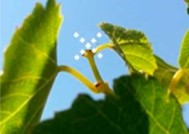
\includegraphics[width=2.08333in,height=\textheight,keepaspectratio]{images/apex0.jpg}
&
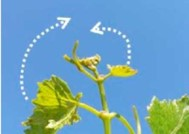
\includegraphics[width=2.08333in,height=\textheight,keepaspectratio]{images/apex1.jpg}
&
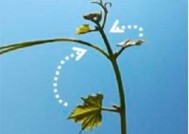
\includegraphics[width=2.08333in,height=\textheight,keepaspectratio]{images/apex2.jpg} \\
L'apex est sec ou à chu & Lorsque les deux dernières feuilles étalées
sont repliées le long de l'axe du rameau, celles-ci recouvrent l'apex. &
Lorsque les deux dernières feuilles étalées sont repliées le long de
l'axe du rameau, celles-ci ne recouvrent pas l'apex. \\
Classe C & Classe R & Classe P \\
\end{longtable}

\subsection{Outils}\label{outils}

La notation peut être réalisée grâce à l'application ApexVigne {[}3,4{]}
disponible sous Android sur
\href{https://play.google.com/store/apps/details?id=ag.GB.apex}{ce lien}
consulté en novembre 2024.

\subsection{Période de mesure}\label{puxe9riode-de-mesure}

Les mesures doivent commencer après la floraison et avant le premier
rognage. Elles sont effectuées toutes les semaines, sauf après un
rognage où un délai d'au moins 1 semaine est nécessaire avant la mesure
suivante pour permettre la reprise éventuelle de la croissance.

\subsection{Aspects pratiques}\label{aspects-pratiques}

La notation est assez rapide, 5 minutes sont nécessaires à une personne
habituée pour évaluer 50 apex.

Traitement des résultats

\section{Variables brutes}\label{variables-brutes}

Les données brutes sont l'ensemble des notes d'apex à chaque
observation.

\section{Variables calculées}\label{variables-calculuxe9es}

Les proportions d'apex dans chaque classe sont calculés et notés
P\textsubscript{C}, P\textsubscript{R} et P\textsubscript{P} (varient
entre 0 et 1). À partir des notations d'apex, il est possible de
calculer des variables élaborées, en particulier l'indice de croissance
et l'indice d'arrêt de croissance.

\subsection{Indice de croissance}\label{indice-de-croissance}

L'indice de croissance (\emph{iC\textsubscript{Apex}}) a été proposé par
{[}4{]}. Il est calculé de la façon suivante :

\[ iC_{Apex} = P_P + 0.5*P_R \]

Cet indice varie entre 0 et 1 : 0 croissance nulle et 1 croissance
active

\subsection{Indice d'arrêt de
croissance}\label{indice-darruxeat-de-croissance}

L'indice d'arrêt de croissance (\emph{IAC}) a été proposé par William
Trambouze {[}2{]}. L'\emph{IAC} varie de 0 (pleine croissance) à 100
(arrêt total de la croissance).

\[ IAC = \frac{100 (1-P_P + P_R + 2P_C)}{3} \]

\begin{tcolorbox}[enhanced jigsaw, leftrule=.75mm, bottomtitle=1mm, toptitle=1mm, colframe=quarto-callout-important-color-frame, toprule=.15mm, opacityback=0, colbacktitle=quarto-callout-important-color!10!white, arc=.35mm, breakable, bottomrule=.15mm, titlerule=0mm, title=\textcolor{quarto-callout-important-color}{\faExclamation}\hspace{0.5em}{Important}, left=2mm, rightrule=.15mm, opacitybacktitle=0.6, coltitle=black, colback=white]

Etant donnée que différents indices synthétiques peuvent être calculés,
il est nécessaire de conserver les données brutes, ou \emph{a minima}
les proportions P\textsubscript{P}, P\textsubscript{R} et
P\textsubscript{C}.

\end{tcolorbox}

\subsection{Date d'arrêt de
croissance}\label{date-darruxeat-de-croissance}

C'est la date à laquelle l'indice de croissance atteint la valeur 0.5.
Elle est déterminée par interpolation entre deux notations d'apex
encadrant la valeur \emph{iC\textsubscript{Apex}} = 0.5.

\section{Interprétation des
résultats}\label{interpruxe9tation-des-ruxe9sultats}

Une relation entre indice de croissance et niveau de contrainte hydrique
potentielle a été établie. L'\emph{IAC} a été mis au point pour le
déclenchement de l'irrigation, il sera plus discriminant en début de
saison, alors que la variation de l'\emph{iC\textsubscript{Apex}} est
plus linéaire.

Compléments d'information

\section{Ressources
complémentaires}\label{ressources-compluxe9mentaires}

\href{https://www.vignevin-occitanie.com/fiches-pratiques/methode-des-apex/}{Fiche
disponible en ligne} sur le site IFV Occitanie

\href{https://www.institut-rhodanien.com/article/fiche-technique-la-methode-des-apex}{Fiche
en ligne} de l'Institut Rhodanien.

\section*{Références}\label{ruxe9fuxe9rences}
\addcontentsline{toc}{section}{Références}

\phantomsection\label{refs}
\begin{CSLReferences}{0}{0}
\bibitem[\citeproctext]{ref-trambouze2009}
\CSLLeftMargin{1. }%
\CSLRightInline{Trambouze, W.; Lovelle-Rodriguez, B.; Jacquet, O. XVIth
international Giesco Symposium.; Davis, California, USA, 2009.}

\bibitem[\citeproctext]{ref-lovelle-rodriguez2009}
\CSLLeftMargin{2. }%
\CSLRightInline{Lovelle-Rodriguez, B.; Trambouze, W.; Jacquet, O.
Évaluation de l'état de croissance végétative de la vigne par la méthode
des apex. \emph{Le Progrès agricole et viticole} \textbf{2009},
\emph{126}, 7788.}

\bibitem[\citeproctext]{ref-brunel2019}
\CSLLeftMargin{3. }%
\CSLRightInline{Brunel, G.; Pichon, L.; Taylor, J.; Tisseyre, B.
\href{https://doi.org/10.3920/978-90-8686-888-9_115}{12th European
Conference on Precision Agriculture}.; Wageningen Academic Publishers:
Montpellier, France, juillet 8 2019; p. 935‑942.}

\bibitem[\citeproctext]{ref-pichon2020}
\CSLLeftMargin{4. }%
\CSLRightInline{Pichon, L.; Brunel, G.; Payan, J.-C.; Tisseyre, B.
Apex-Vigne: A mobile application to facilitate the monitoring of growth
and estimate the water status of the viticulture plots. \emph{IVES
Technical Reviews, vine and wine} \textbf{2020},
doi:\href{https://doi.org/10.20870/IVES-TR.2020.3558}{10.20870/IVES-TR.2020.3558}.}

\end{CSLReferences}




\end{document}
